\section{Grenzen selbststeuernder produktionslogistischer Prozesse}
\label{sec:Grenzen}

Im vorherigen Kapitel wurden die erarbeiteten Möglichkeiten der
selbststeuernden Prozesse aus dem Beispiel einem vergleichbaren Prozess der
Fließfertigung gegenüber gestellt. Hieraus ergaben sich Vorteile für selbst
steuernde Prozesse, die im Nachfolgenden auf Ihre Grenzen untersucht werden
sollen.

Die Grenzbetrachtung basiert auf der folgenden Darstellung aus Evolution der
Logistik (\citet{evolution2007}):

\begin{figure}[htb] 
\centering
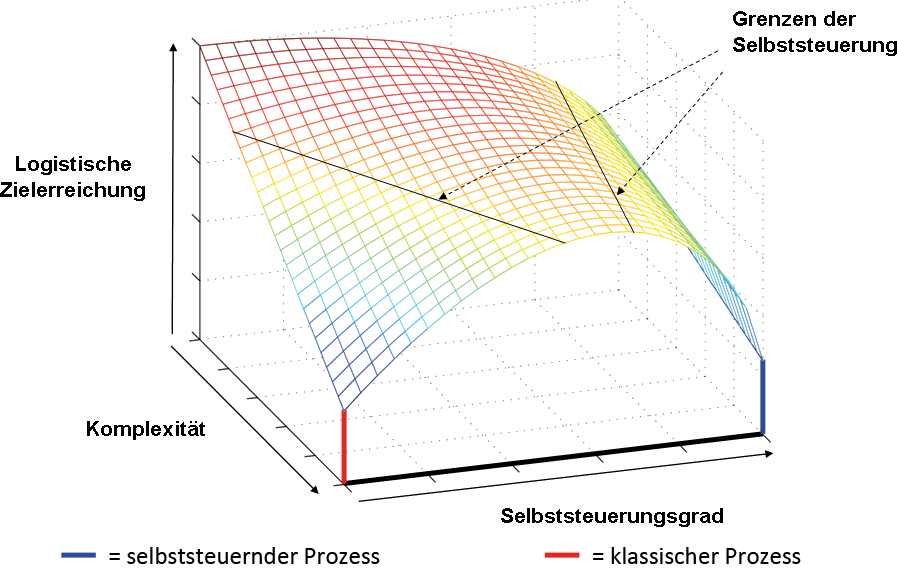
\includegraphics[width=1.0\textwidth]{Grenzbetrachtung.png}
\caption[Grenzbetrachtung]{Grenzen selbststeuernder Prozesse\protect\footnotemark}
\label{fig:Grenzbetrachtung}
\end{figure}
\footnotetext{entnommen aus \citet[S.~3]{evolution2007}}

Im Folgenden werden, die in der Darstellung unterstellten Grenzen der
Selbststeuerung untersucht. Die dargestellten Grenzen lassen sich dabei in drei
Mängel unterscheiden, die bei bestimmten Produktionssituationen vorliegen:

\begin{itemize}
  \item Fehlender Mehrwert bei geringer Komplexität
  \item Fehlender Merhwert bei Make-to-Stock-Produkten
  \item Kontrollverlust als Grenzen der Selbststeuerung
\end{itemize}

Die Unterscheidung in diese drei Grenzbereiche werden in den nachfolgenden 
Abschnitten näher erläutert.

\subsection{Fehlender Mehrwert bei geringer Komplexität}
\label{sec:GrenzenKomplexitaet}

Zunächst kann aus der dargestellten Abbildung entnommen werden, dass die Autoren
Scholz-Reiter, de Beer, Böse und Windt der Meinung sind, dass der Mehrwehrt von
Selbststeuerung für logisitische Prozesse mit abnehmender Komplexität der
Produktionsprozesse ebenfalls abnimmt. Bei einfachen logistischen Prozessen
übersteigt der Aufwand der Implementierung und des Betriebes von autonomen
Produktionsanlagen den Nutzen, den diese mit sich bringen. Bezogen auf das
eingangs erwähnte Fallbeispiel lässt sich diese Meinung einfach verdeutlichen:

Angenommen die Produktion der PKW-Rücklichter ist eine reine Massenproduktion
aus wenigen Einzelteilen und ohne besondere Variantenvielfalt, dann kann die
Produktion als wenig komplex eingestuft werden. Die Steuerung der
Produktionsanlagen weist in diesem Fall eine ebenso geringe Komplexität auf, da
die Eingangsgrößen des Prozesses deterministisch geplant werden können. Wir sind
der Meinung, dass in einem solchen System die Mehrwehrte von selbststeuernden
Prozessen, im Gegensatz zu zentral gesteuerten Prozessen, nicht signifikant
sind.

Diese Meinung begründen wir mit dem fehlenden Bedarf nach autonomer
Entscheidungsfindung. Da die Steuerung der Produktionsanlagen wenig komplex ist
kann sie auch von zentralen Systemen übernommen werden. Ein
Geschwindigkeitsvorteil bei der autonomen Entscheidungsfindung bleibt aus. Auch
die Steuerung der Produktionswege zur Optimierung der Maschinenauslastung und
die Reaktion auf Maschinenausfälle kann durch eine zentrale Steuerung
zeitgerecht realisiert werden.

\subsection{Fehlender Mehrwert bei Make-to-Stock-Produktionen}
\label{sec:GrenzenMakeToStock}

Produktionsabläufe bei denen die Produkte auf Vorrat produziert werden, werden als "`make-to-stock"' bezeichnet. Bei dieser 
Produktionsform ist der Mehrwert von selbststeuernden Prozessen aus unserer Sicht nicht relevant. 
Diese Meinung begründen wir mit dem fehlenden Bedarf nach Flexibilität in dieser Produktionsform.
Analog zur Annahme im vorherigen Kapitel kann an dieser Stelle angenommen werden, dass das PKW-Rücklicht als ein 
Massenprodukt in einem Push-Prozess\footnotemark auf Vorrat produziert werden. 
Die Produktionsmengen von diesen make-to-stock-Produkten 
werden anhand von deterministischen Marktkennzahlen geplant und hängen damit nicht von variablen Kundenwünschen ab. Der 
Produktionsablauf kann vorrausgeplant werden und muss nicht flexibel auf Änderungen reagieren. Ein gesteigerter Bedarf 
nach Flexibilität ist nicht vorhanden.
Darüber hinaus führt planerische Sicherheit der Produktion dazu, dass der Mehrwert der optimalen Maschinenauslastung bei 
selbststeuernden Prozessen auch mit zentraler Steuerung erreicht werden kann. Die optimale Auslastung aller Maschinen kann 
in diesem Beispiel auf Grund der vorher geplanten Produktionsmenge zentral berechnet und gesteuert werden.

\footnotetext{Erläuterung Push-Prozess}

Am Ende dieser Betrachtung bleibt aber festzuhalten, dass selbsteuernde Prozesse bei komplexen make-to-stock-Produktionen 
eine Erhöhung der Ausfallsicherheit mit sich bringen können. Dieser vergleichsweise geringe Mehrwehrt rechtfertigt aber 
unserer Sicht nicht den Aufwand, der für eine Umstellung auf eine selbststeuernde Produktion anfällt.

\subsection{Kontrollverlust bei vollständiger Selbststeuerung}
\label{sec:GrenzenKontrollverlust}

Als letzter Aspekt der Grenzbetrachtung wird eine vollständig autonome
Produktionssteuerung betrachtet. Aus der vorgestellten Abbildung wird
ersichtlich, dass die Autoren Scholz-Reiter, de Beer, Böse und Windt bei
vollständiger Selbststeuerung eine geringe logistische Zielerreichung
voraussagen. Dieser Meinung stimmen wir ebenfalls mit nachfolgender Begründung
zu:

Bei einer vollständigen Autonomie der Produktionsprozesse in einem
heterarchischen System bleibt keine Kontrollmöglichkeit bzw. zentrale
Eingriffsmöglichkeit mehr offen. Das Fehlen einer zentralen
Eingriffsmöglichkeit führt bei Änderungen von Entscheidungsparametern zu
produktionslogistischen Fehlern. \hfill \\
Es wird dazu zunächst angenommen, dass die Auswahl der PKW-Rücklichtblende im
vorgestelltem Fallbeispiel von einer Information abhängt, die an den
Rücklichtern angebracht ist. Ändert sich dieser Entscheidungsparameter, das
heißt die Entscheidung wird beispielsweise aufgrund einer anderen Information
getroffen, muss diese Veränderung jeder autonomen Entscheidungseinheit separat
mitgeteilt werden. Aufgrund der fehlenden Möglichkeit diese Änderung zentral zu
verbreiten entscheidet jede Einheit zunächst falsch. Diese falsche
Entscheidungen können dazu führen, dass viele Produkte fehlerbehaftet
produziert werden oder die Produktion angehalten werden muss. Eine vollständige
Autonomie dezentraler Einheiten ist aus diesen Gründen nicht sinnvoll.

\clearpage